\section{MTCNN Face Detection}
\label{MTCNN}
Bei Multi-task Cascaded Convolutional Network handelt es sich um ein Verfahren dass bei der Detektion von Gesichtern auch deren Ausrichtung berücksichtigt wird, um so bessere Ergebnis zu erzielen.
\subsection{Anforderungen}
Sein Einsatzgebiet ist die Vorverarbeitung eines Frames für die spätere Auswertung. Somit soll dieser Schritt von einem möglichst robusten Verfahren zur Detektion von Gesichtern durchgeführt werden.\\
Dabei wird auf recht großen Bild gearbeitet mit verhältnismäßig kleinen und verschieden großen Gesichtern.\\
Außerdem sollte das Verfahren ausreichend schnell sein, da es sich hierbei nur um ein Vorverarbeitungsschritt handelt und zur Beschleunigung der späteren Berechnung beitragen soll.
\subsection{Die 3 Stufen der Verarbeitung}
Für die gute Detektionsqualität sorgt die dreistufige Verarbeitung auf der Bildpyramide. Bei der Bildpyramide handelt es ich um ein in verschiedenen Größen skaliertes Bild, damit der Gesuchte Inhalt in der gewünschten Auflösung abgebildet ist, ohne dass etwas über den Inhalt bekannt ist.\\
Dies ist von Vorteil, damit das CNN auf eine feste Größe von Gesichtern optimiert werden kann, um neben dem möglichen Farbverläufen, durch die Skalierung das Lernen nicht zusätzlich zu erschweren.
\begin{figure}
	\centering
	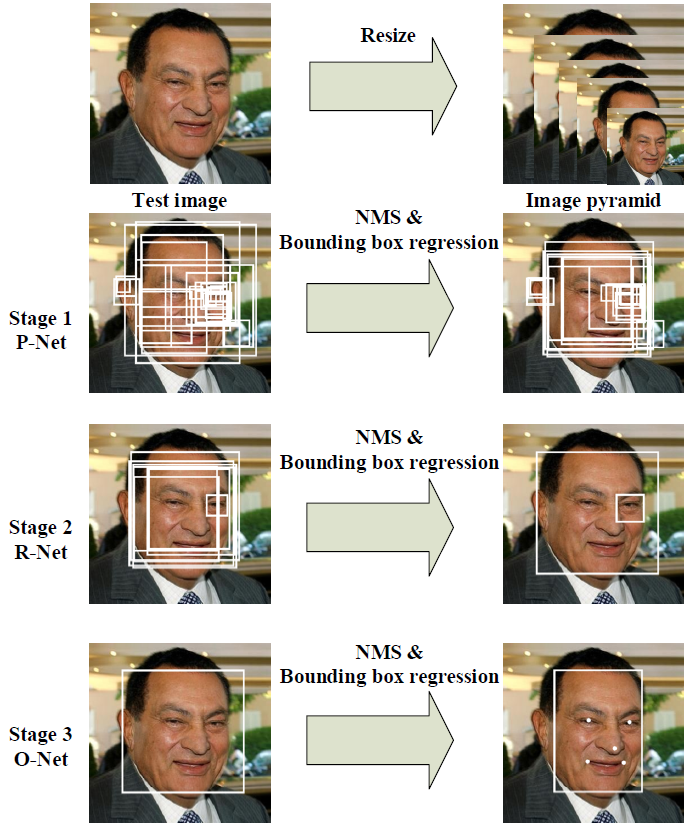
\includegraphics[width=0.5\linewidth]{img/MTCNN_Step}
	\caption{Darstellung des Funktionsablaufes von MTCCN\cite{MTCCN}}
	\label{img_MTCNN_Step}
\end{figure}
\subsubsection{Stufe 1}
Beim ersten Verarbeitungsschritt erden alle Bereiche eines Bilds gesucht, in denen möglicherweise ein Gesicht zu sehen ist. Dazu wird zuerst ein einfaches CNN eingesetzt und die Ergebnisse, die sich sehr stark überlappen, zusammengefasst.\\
Für die Detektion wird von einem CNN, dem sogenannte Proposal Network (P-Net), eingesetzt und sehr viele Bounding-Boxen ermittelt. Diese werden nun mit einem NMS ausgedünnt, um die am stärksten überlappenden Bounding-Boxen zusammen zu fassen.
\subsubsection{Stufe 2}
Anschließend werden die möglichen Bereiche mittels eines weiten CNN analysiert, damit alle Nicht-Gesichtsbereiche erkannt und entfernt werden können.\\
Dies wird von dem Refine Network (R-Net) übernommen und anschließend die möglichen Bounding-Boxen mittels NMS weiter reduziert.
\subsubsection{Stufe 3}
Der letzte Schritt wird von einem deutlich genaueren CNN übernommen, um ein Gesicht zu detektieren, dem sogenannten Output Network (O-Net). Womit die resultierenden exakten Boxen und 5 Landmarks ermittelt werden.
\subsection{Qualität}
MTCNN Face Detection ist bei der Zuverlässigkeit im Verglich zu anderen bekannten Verfahren überlegen, siehe \autoref{img_MTCNN_quality} und zudem Echtzeit fähig. Im Test-Datensatz sind auch Gesichtern mit einer Größe von $20\times 20$ enthalten und wurden erfolgreich erkannt.\\
Somit sind alle Anforderungen erfüllt um mit diesem Verfahren den vorhanden Frame für die nachfolgenden Berechnungen vorzubereiten, daher wird es auch hier eingesetzt.
\begin{figure}
	\centering
	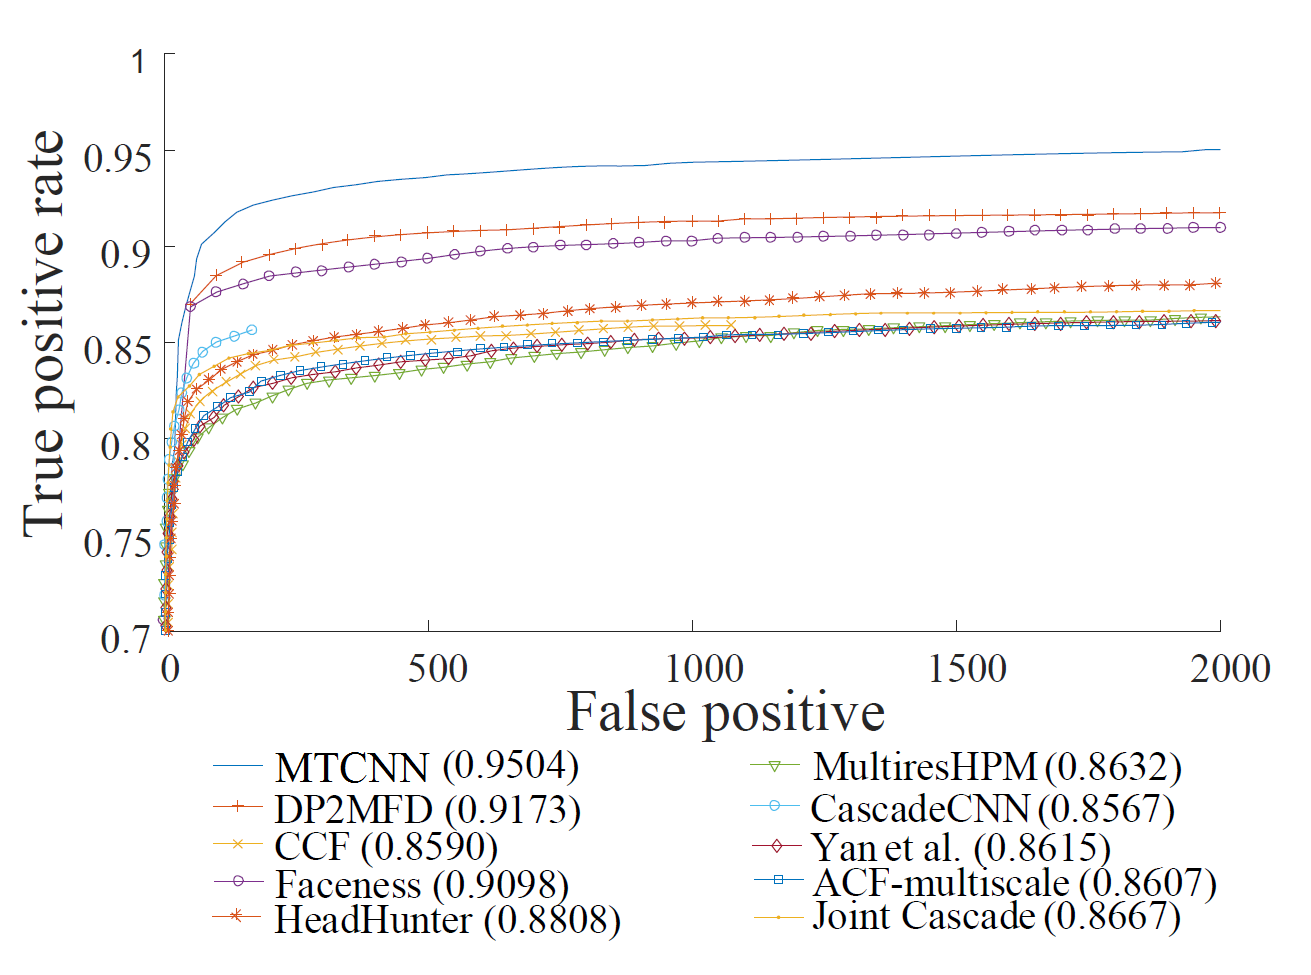
\includegraphics[width=0.5\linewidth]{img/MTCNN_quality}
	\caption{normale blaue Linie\cite{MTCCN}}
	\label{img_MTCNN_quality}
\end{figure}
%Joint Face Detection and Alignment using Multi-task Cascaded Convolutional Networks